\chapter{\mc 足動作検知のための\rm BCI}
この章では足動作検知を目標として構築したBCIについて説明する。
BCIは個人の脳波の解析と、信号処理、特徴量抽出器。分類器を組み合わせて構築した。

\section{\mc 計測した\rm EEG\mc について}
まず、被験者が8秒間静止(以後rest状態)と
8秒間足動作(以後walk状態)を8サイクル繰り返したときのEEGを計測した。
被験者はリラックスできる椅子に着席した状態で前方に配置されたディスプレイの
指示に従って動作を行った(図\ref{fig:asibumi})。
ただし、8サイクル中最初の1サイクルについてはフィルタの応答の特性上、
EEGの解析には適さないと判断し、解析時には除外した。
従って以後の解析で用いられるのは7サイクル分のEEGである。
EEGの計測機器としてはg.tec社のg.USBamp(図\ref{fig:usbamp})を用い、ウェット式の電極を採用した。
ウェット式では頭皮と電極の間に導電性のジェルを注入することでEEGを計測する。
EEGの計測時にはジェルの注入を行いながら、すべての電極に関して電極インピーダンスが\(5k\Omega\)
以下になったことを確認した。
またサンプリング周波数は128Hzとした。
\begin{figure}
    \centering
    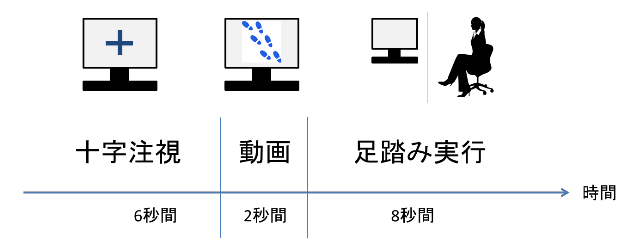
\includegraphics[width=13cm]{images/asibumi.png}
    \caption{EEG計測時のタイムスケジュール}
    \label{fig:asibumi}
\end{figure}
\begin{figure}
    \centering
    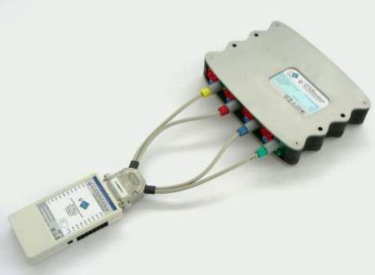
\includegraphics[width=8cm]{images/usbamp.png}
    \caption{g.tec社のg.USBamp}
    \label{fig:usbamp}
\end{figure}

計測に用いた電極の個数は5つであり、Cz、C1、C2、CPz、FCz電極である。
Cz電極は足に関する運動野が脳の頭頂部に存在するため選出し、
スモールラプラシアンフィルタが適用できるように残りの4つを選出した(図\ref{fig:smalllap})。
また、EEGの計測時には定常成分とERDとは無関係な高周波成分を削除するために
通過帯域を0.3Hzから36Hzとした2次のバタワースバンドパスフィルタを用いた。

\section{\rm EEG \mc の解析とBCIの構築}
\subsection{\mc スペクトル密度推定による\rm ERD\mc の確認}
まずCz電極で計測されたEEGと
Cz電極に対してスモールラプラシアンフィルタを用いた際の
EEGを図\ref{fig:eegsub1}に添付する。
ここで、\(x_{A}(t)\)はA電極によって計測された波形であるとして
Cz電極に対してスモールラプラシアンフィルタを用いた際の波形\(z(t)\)は以下である。
\begin{equation}
    z(t) = x_{Cz}(t) - \frac{1}{4}(x_{C1}(t) + x_{C2}(t) + x_{FCz}(t) + x_{CPz}(t))
\end{equation}
スモールラプラシアンフィルタの定義から、
頭皮上でCz電極に際立った電位分布が獲得されていることが期待できる。

\begin{figure}
    \centering
    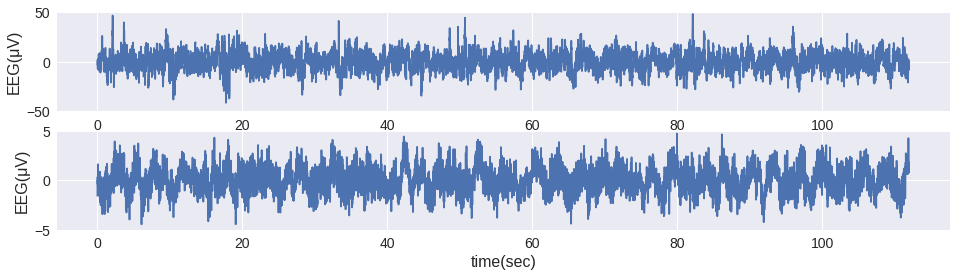
\includegraphics[width=13cm]{images/eeg_sub1.png}
    \caption{Cz電極のEEG(上)とスモールラプラシアンフィルタを用いたEEG(下)}
    \label{fig:eegsub1}
\end{figure}
% \begin{figure}
%     \centering
%     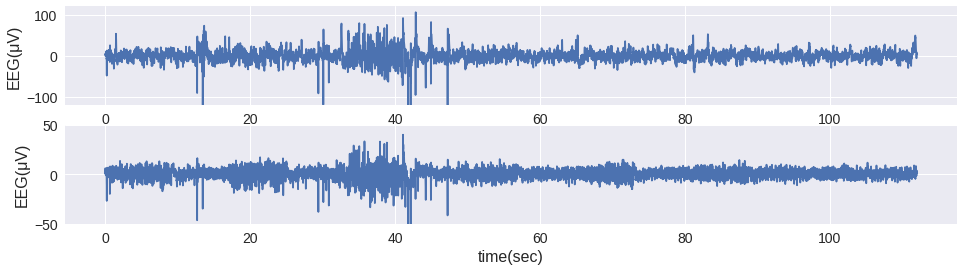
\includegraphics[width=13cm]{images/eeg_sub2.png}
%     \caption{被験者2のCz電極のEEG(上)とスモールラプラシアンフィルタを用いたEEG(下)}
%     \label{fig:eegsub2}
% \end{figure}

% 続いて、PCAとICAによる空間フィルタの設計を試みた。
% それぞれのフィルタから得られる各被験者のEEGの波形を図\ref{fig:bss1}と図\ref{fig:bss2}に示す。
% が\label{section:BSS}にて述べた問題のために、
% 得られた信号のいずれが重要であるかの判断を行うことができなかった。

次にスモールラプラシアンフィルタを用いたEEGの
rest状態(8秒間)の波形とwalk状態(8秒間)の波形それぞれに対してパワースペクトル密度推定を行った。
スペクトル密度推定には1秒間(128点)の時間窓を用いたウェルチのオーバラップ法を利用し、
オーバラップは0.5秒(64点)とした。
rest状態とwalk状態は計7回繰り返し行なっているため図\ref{fig:allERDs}に
7回分すべてのスペクトル密度の比較を示す。
また図\ref{fig:walkERD}に7回分の平均を示す。
ERDの生ずる周波数帯域は個人差があるとされるが、
\(\mu\)律動(8-12Hz)や\(\beta\)律動(18-26Hz)で
パワーの減少が観測できる報告があり\cite{erdfreq}、また\cite{Beta波によるBCI}では
6-40Hzの領域に渡ってERDを検知しBCIを構築した例がある。
概ね先行研究において観測されている周波数帯域でwalk時のパワーの減少が確認された。
\begin{figure}
    \centering
    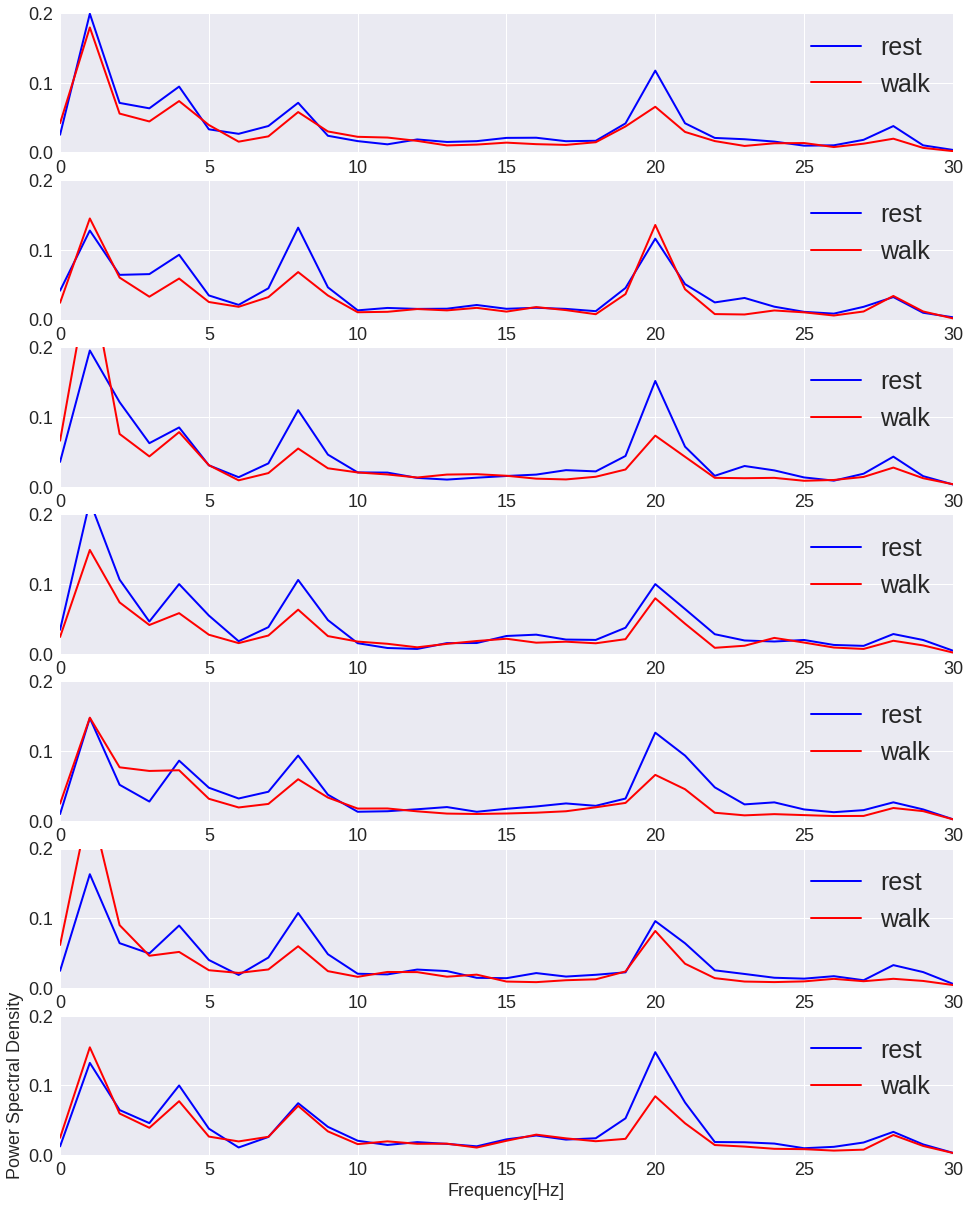
\includegraphics[width=13cm]{images/allERDs}
    \caption{rest時とwalk時のパワースペクトル密度の比較}
    \label{fig:allERDs}
\end{figure}
\begin{figure}
    \centering
    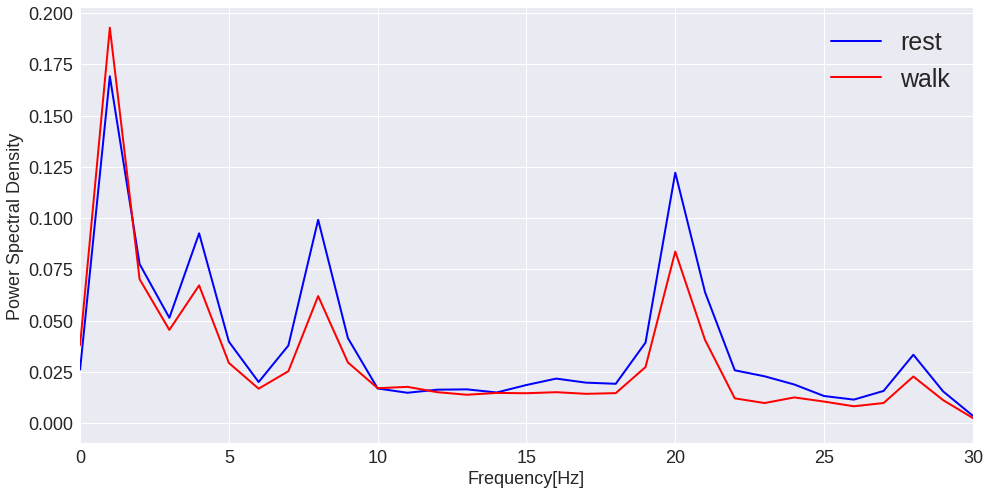
\includegraphics[width=13cm]{images/walkERD}
    \caption{rest時とwalk時のパワースペクトル密度の平均(7回分)の比較}
    \label{fig:walkERD}
\end{figure}

しかし、平均(図\ref{fig:walkERD})を確認すると
4、8、20Hz付近で際立ったパワーの減少が見られるが、
個々のスペクトル密度(図\ref{fig:allERDs})は必ずしもパワーの減少が
すべてのサイクルで同様に確認できることを示してはいない。
例として20Hzで際立ったパワーの減少(ERD)が生ずると考えた場合には、
図\ref{fig:allERDs}の上から2番目に関しては検知ができないことになる。
従って、ERDを検知してBCIを動作させることを考える場合には、
複数の周波数帯域のパワーを総合的に評価する必要があると考えられる。

また、パワースペクトル密度の絶対値を評価するよりも
rest状態とwalk状態の相対的なパワーの差の方が重要であることが言える。
例として、図\ref{fig:walkERD}から20Hzのパワースペクトル密度が0.1以下になった場合に
walk状態であると判定するBCIは図\ref{fig:allERDs}の下から二番目のグラフの
rest状態をwalk状態と判定することになる。
パワーの絶対値がさほど重要な指標にならないことは、
EEGの計測が電極のインピーダンス(ジェルの塗布状況)や
頭皮のインピーダンス(皮脂や毛髪)に左右されることからも想定されることである。

従ってERDを検知するためには複数の周波数帯域に跨って、
rest状態とwalk状態の相対的なパワーの変化に着目する必要があると考えた。


\subsection{\mc 足動作検知のための信号処理}
解析結果に基づいて、EEGに対して以下の信号処理によって特徴量を獲得した。
\begin{enumerate}
    \item 2種類のバンドパスフィルタ:通過帯域を3-14Hzと13-33Hz
    \item スモールラプラシアンフィルタ:Cz電極に適用
    \item バーグ法によるスペクトル密度推定:時間窓を1秒(128点)、オーバラップ127点
    \item ローパスフィルタ:スペクトル密度の時間変化の平滑化
    \item ハイパスフィルタ:パワースペクトル密度の時間変化の定常成分カット
\end{enumerate}
上記の処理における1.〜5.の概略図を図\ref{fig:footBCI}に示す。
\begin{figure}
    \centering
    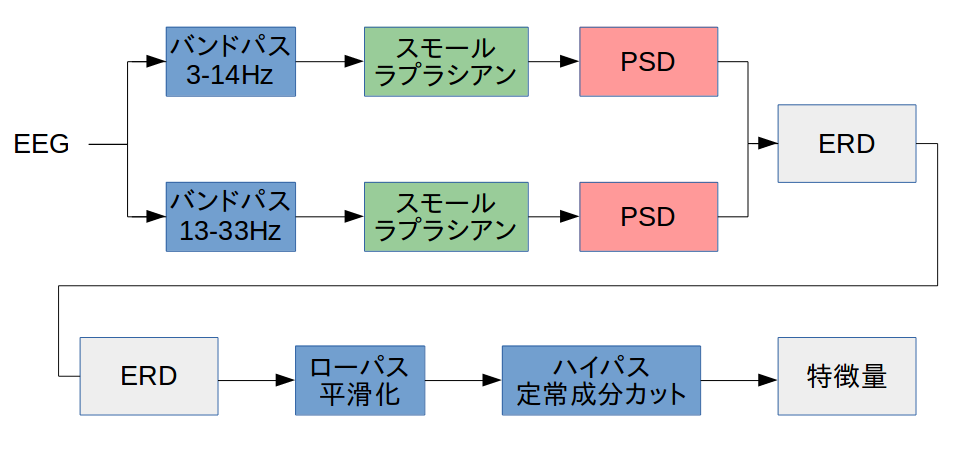
\includegraphics[width=13cm]{images/prepro.png}
    \caption{EEGから特徴量を獲得する処理の流れ}
    \label{fig:footBCI}
\end{figure}
1.〜3.の処理では2種類のバンドパスフィルタを通過したEEGに対してそれぞれスペクトル密度推定が行われる。
3−14Hzのバンドパスフィルタを通過した波形に関しては、パワースペクトル密度の4-13Hzのみを利用し、
13−33Hzのバンドパスフィルタを通過した波形に関しては、パワースペクトル密度の15-32Hzのみを利用した。
この着目する帯域は、EEGの\(\alpha\)律動及び\(\mu\)律動、\(\beta\)律動などの周波数帯域と
解析したEEGのピークの位置を加味し、経験的に定めた。
時間窓は1秒間であるため周波数分解能は1Hzであり、各時間窓において計28の特徴量が得られる。
時間窓は1サンプル点ずつ移動させるため、1/128秒毎に28次元の特徴量が出力される。
図\ref{fig:nofilterERD}に1.〜3.の処理を施した出力を添付する。
\begin{figure}[p]
    \centering
    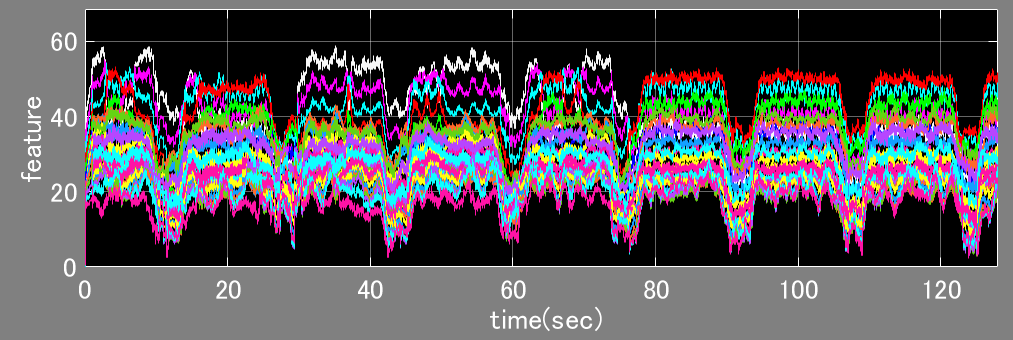
\includegraphics[width=13cm]{images/feature_sub1_nofilter.png}
    \caption{28個の特徴量の時間変化}
    \label{fig:nofilterERD}
\end{figure}
図\ref{fig:nofilterERD}からは、
特徴量が全体的に減少している様子が8回分観測できる。
また特徴量はパワースペクトル密度の時間変化に他ならないため、
特徴量の減少はERDであり8回の足動作に由来していると考えられる。

次に、特徴量の変化がrest状態とwalk状態において際立つことが重要であり、
同一状態においては変化が少ない方が好ましいことを考慮し
4.ローパスフィルタによる平滑化を行った。この処理によって、
状態が切り替わる程の大きな特徴量の変化が強調される(図\ref{fig:lfilterERD})。
\begin{figure}[p]
    \centering
    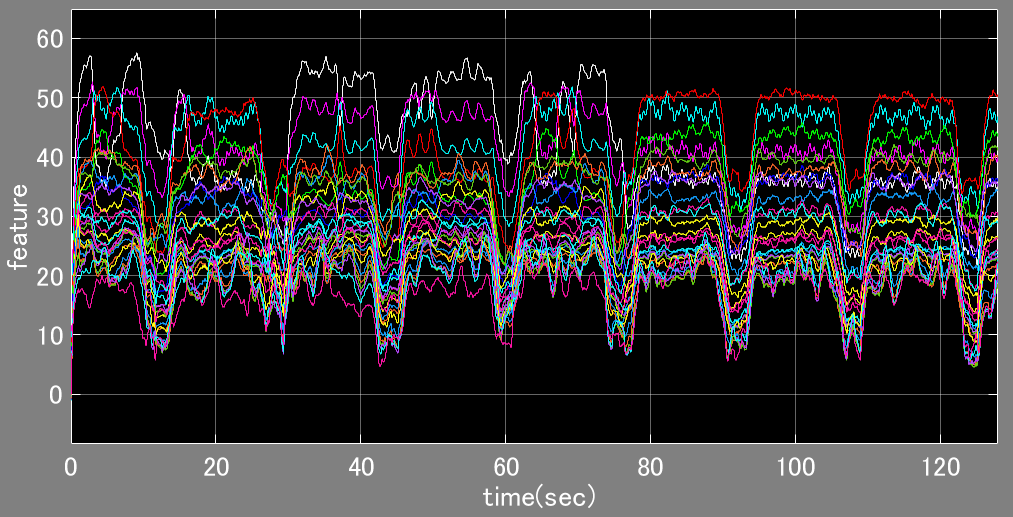
\includegraphics[width=13cm]{images/feature_sub1_l.png}
    \caption{ローパスフィルタを追加した28個の特徴量の時間変化}
    \label{fig:lfilterERD}
\end{figure}

また、ERDを検知する場合には
rest状態とwalk状態の各状態間のパワースペクトル密度の相対的差異が重要である
と考えられることを前述した。
同時に、分類器にとっても相対的差異のみが重要であり絶対値は影響しないことを考慮し、
5.ハイパスフィルタによって定常成分をカットした(図\ref{fig:filterERD})。
\begin{figure}[p]
    \centering
    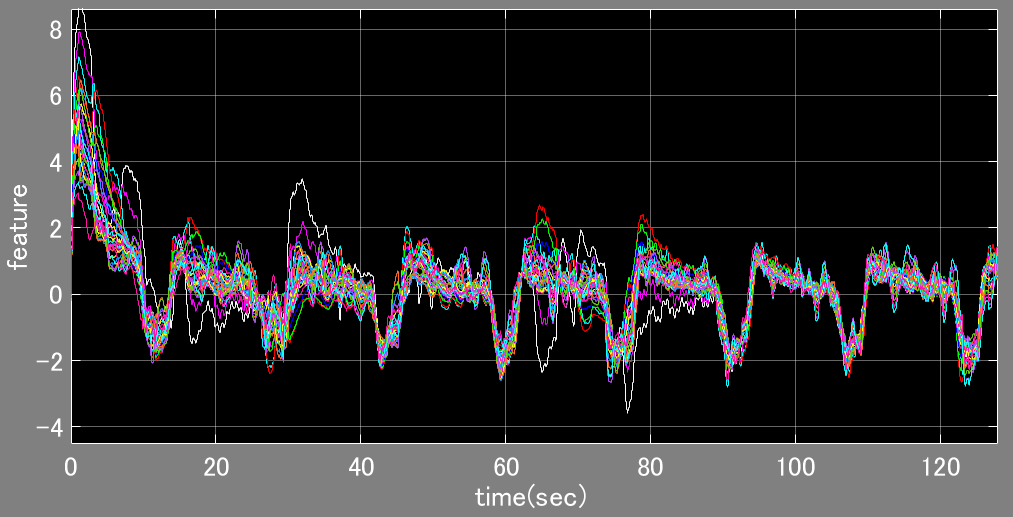
\includegraphics[width=13cm]{images/feature_sub1.png}
    \caption{ローパスフィルタとハイパスフィルタを追加した28個の特徴量の時間変化}
    \label{fig:filterERD}
\end{figure}

バーグ法によるスペクトル密度推定値をピリオドグラムに置き換え、
同様の処理を行った際の特徴量の時間変化を図\ref{fig:fftERD}に示す。
またバーグ法をウェルチのピリオドグラム法で置き換えた際の特徴量の時間変化を
図\ref{fig:welchERD}に示す。
いずれもスペクトル密度推定として広く用いられる方法であるが、バーグ法を用いた
場合のスペクトル密度の時間変化(図\ref{fig:filterERD})は
特徴量(ERD)が目視できるほどに強調されていることが分かる。

\begin{figure}[tp]
    \centering
    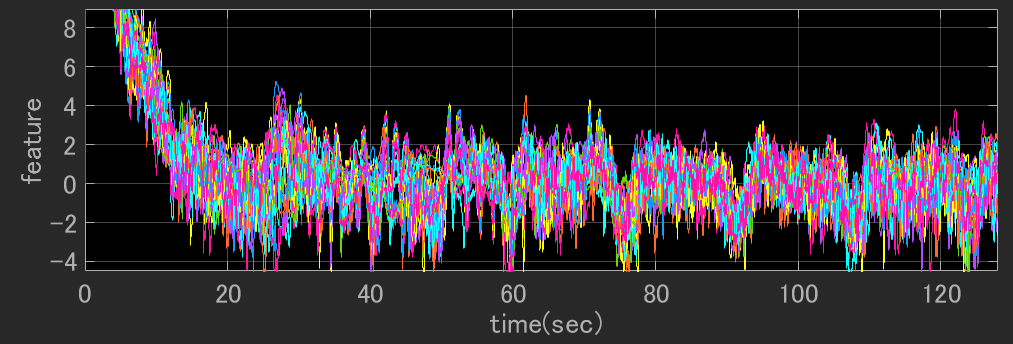
\includegraphics[width=13cm]{images/feature_sub1_fft.png}
    \caption{ピリオドグラムを用いた28個の特徴量の時間変化}
    \label{fig:fftERD}
\end{figure}
\begin{figure}[tp]
    \centering
    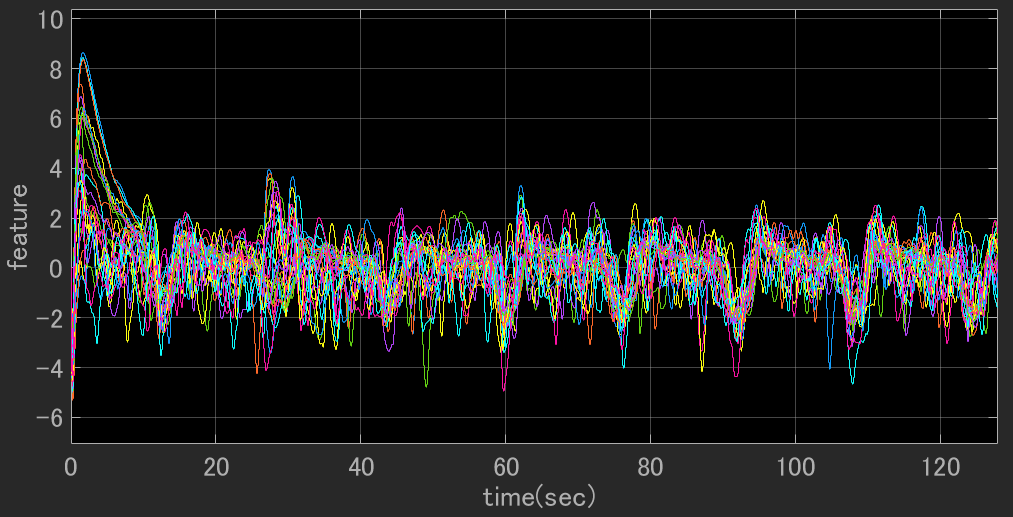
\includegraphics[width=13cm]{images/feature_sub1_welch.png}
    \caption{ウェルチのピリオドグラム法を用いた28個の特徴量の時間変化}
    \label{fig:welchERD}
\end{figure}

\subsection{\mc 分類器}
ここまでの処理によって得られた特徴量の次元は28であり、
以後\(x_i \in \mathbb R^{28}\)と表記する。
ここに\(i\)はサンプル時刻を表すインデックスである。
\(x_i\)はサンプル時刻\(i\)における特徴量を格納しており、
特徴量はERDを強調するための処理が施されたものである。
仮に特徴量\(x_i\)を引数としてrest状態かwalk状態を識別する分類器\(y_i=f(x_i)\)を、
\ref{section:discriminant}で述べた手法によって構築することを考えた場合には、
時刻の情報を完全に破棄して各時刻の\(x_i\)に対して個々に分類を行うことになる。
各点の正解ラベルは
EEG計測時のrest状態を\(0\)、walk状態を\(1\)とした(図\ref{fig:targetsignal})。
\begin{figure}[tp]
    \centering
    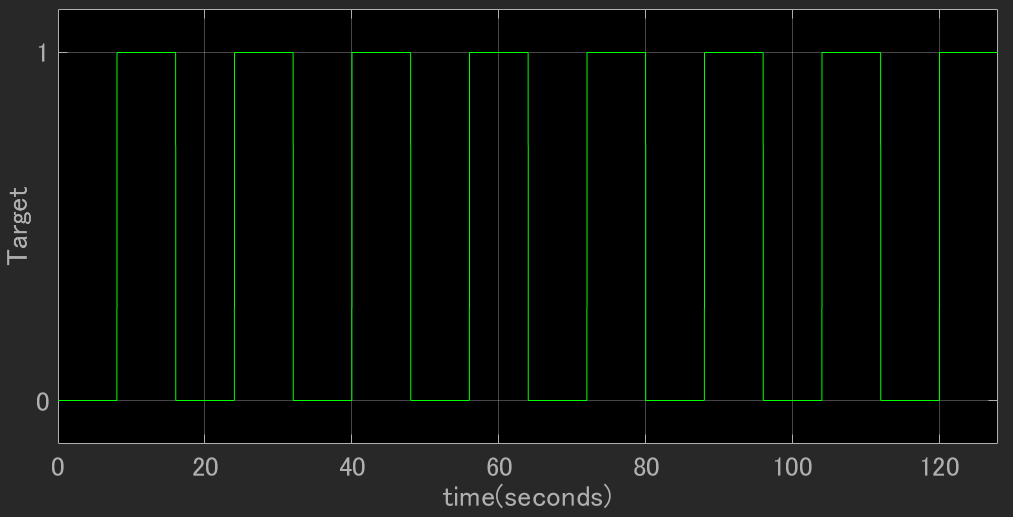
\includegraphics[width=13cm]{images/targetsignal.png}
    \caption{学習時の教師信号(0:rest状態、1:walk状態)}
    \label{fig:targetsignal}
\end{figure}

ただし、
フィルタの特性上EEG計測時の最初のサイクル(0〜16秒)は
学習データとしても検証データとしても用いないこととし、
利用するのは114秒間(16秒〜128秒)で
データ点数は14336点(\(i=1,\cdots,14336\))とする。

\subsubsection{\mc バーグ法による特徴量を用いた分類}
まず、バーグ法により推定されたパワースペクトル密度から得た特徴量を用いて、
ロジスティック回帰による分類を行った。
7交差検証によりAccuracyを算出した結果、
ロジスティック回帰では0.826となった。
続いて、同日に同一被験者から計測したEEGを用いて
抽出した特徴量(14336点)に対しての
学習済モデルのテストAccuracyは0.729となった。

交差検証時に比べ著しい性能の低下が見られる。
ロジスティック回帰にはハイパーパラメータが用いられていないため、
同一被験者であっても新規のEEGに対しては上手く
特徴量が得られていない可能性が示唆される。

EEGの場合は同一被験者であり、仮に脳活動がほとんど等しくとも
頭皮やジェルの状況に応じて計測されるEEGの波形には差異が存在することが想定される。
従って獲得された28個の特徴量のうちのいずれかが、
訓練データとテストデータの間で大きく変化している場合には分類器の性能低下が起こる。
そこで、28個の特徴量の中から分類に関連する重要な次元を選定することとした。

次元削減として用いられるPCAでは変換先で各成分が無相関となるように変換が行われる。
すなわち変換前において相関のある成分は適切な線型結合によって1つの成分に集約される。
今回の場合はERDを抽出することから開始したために、
28次元の特徴量の各成分は明らかに相関性を有しており(図\ref{fig:filterERD})、
一方で期待されるERDの挙動とは異なる波形も見受けられる。
PCAによって不要な成分を削除することで、分類器のテストデータへの性能の向上を試みた。

結果として、次元削減によって28次元を2次元へ変換した場合には
ロジスティック回帰の交差検証Accuracyは0.787となった。
一方でテストAccurcyは0.842となった。
交差検証の結果はPCAを用いる前に比べて悪化しているが、
テストの結果は向上した。
この結果から28次元から2次元に削減された際に、
削除された次元26次元に過学習の要因が含まれていたものと推測できる。

\subsubsection{\mc ウェルチ法特徴量を用いた分類}
次に、ウェルチ法によって推定されたパワースペクトル密度から得た特徴量を用いて、
ロジスティック回帰による分類を行った。
7交差検証によりAccuracyを算出した結果、
ロジスティック回帰では0.889となった。
続いて、同日に同一被験者から計測したEEGを用いて
抽出した特徴量(14336点)に対しての
学習済モデルのテストAccuracyは0.849となった。
また、PCAを用いた次元削減による分類を行った場合のAccuracyは
交差検証で0.758、テストで0.846となった。
表\ref{table:meanacc}に分類手法(ロジスティック回帰をLRと表記)と
スペクトル密度推定の手法の組み合わせに対するテストAccuracyの表を添付する。

\begin{table}[t]
\centering
\caption{テストAccuracyの比較}
    \begin{tabular}{|c|c|c|} \hline
        分類手法\解析手法 & バーグ & ウェルチ \\ \hline
        LR &  0.729  & 0.849  \\ \hline
        PCA + LR & 0.842  & 0.843  \\  \hline
        LDA & 0.829  & 0.839  \\  \hline
    \end{tabular}
    \label{table:meanacc}
\end{table}

\subsection{考察}
この結果は想定外のものであり、
バーグ法によって抽出された特徴量である図\ref{fig:filterERD}に比べ、
ウェルチ法によって抽出された特徴量である図\ref{fig:welchERD}の方が
一見、粗悪な特徴量に見えるためである。
しかし、バーグ法とウェルチ法の特徴量のいずれも
PCAによる第一主成分は極めて似た波形(相関係数0.875)である(図\ref{fig:burgPCA}、図\ref{fig:welchPCA}、図\ref{fig:burgwelchPCA})。

バーグ法で得られた特徴量に関しては、
第一主成分が図\ref{fig:burgPCA}の波形になることは
図\ref{fig:filterERD}を見れば計算前から想定ができる(
元来、ERDを可視化するために構築した信号処理であるため)。
一方ウェルチ法で得られた特徴量(図\ref{fig:welchERD})
から明確にERDを見出すことは難しいが、
第一主成分が図\ref{fig:welchPCA}の波形として得られ
ERDが潜在していたことが明らかになった。
\begin{figure}[p]
    \centering
    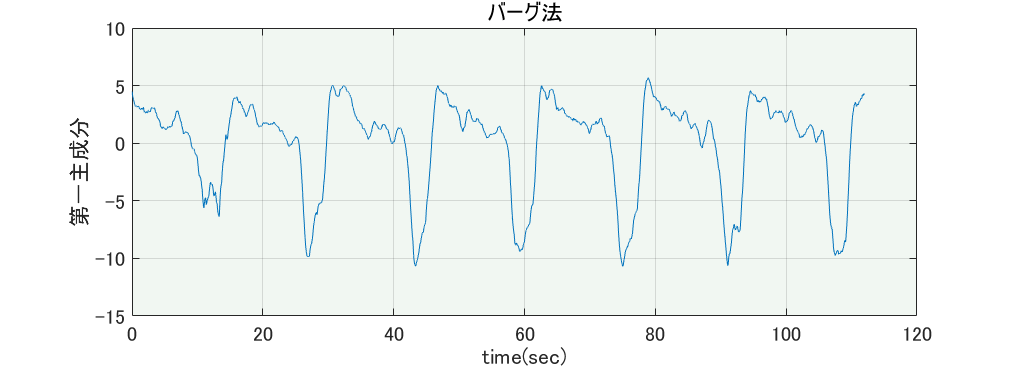
\includegraphics[width=13cm]{images/burgPCA.png}
    \caption{バーグ法で得られた特徴量の第一主成分}
    \label{fig:burgPCA}
\end{figure}
\begin{figure}[p]
    \centering
    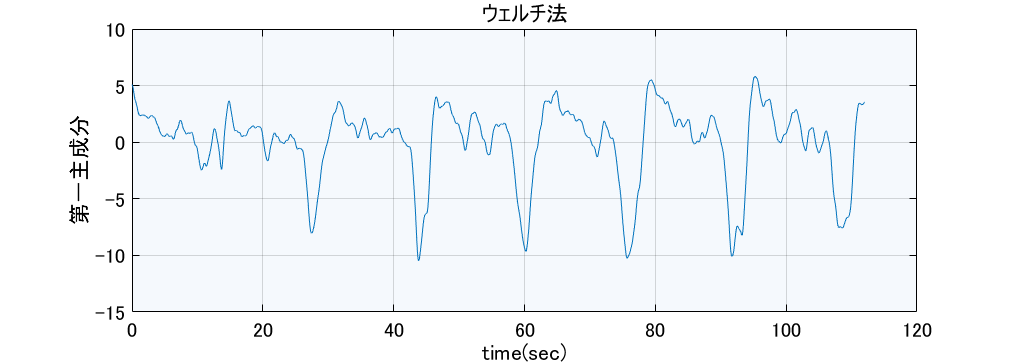
\includegraphics[width=13cm]{images/welchPCA.png}
    \caption{ウェルチ法で得られた特徴量の第一主成分}
    \label{fig:welchPCA}
\end{figure}
\begin{figure}[p]
    \centering
    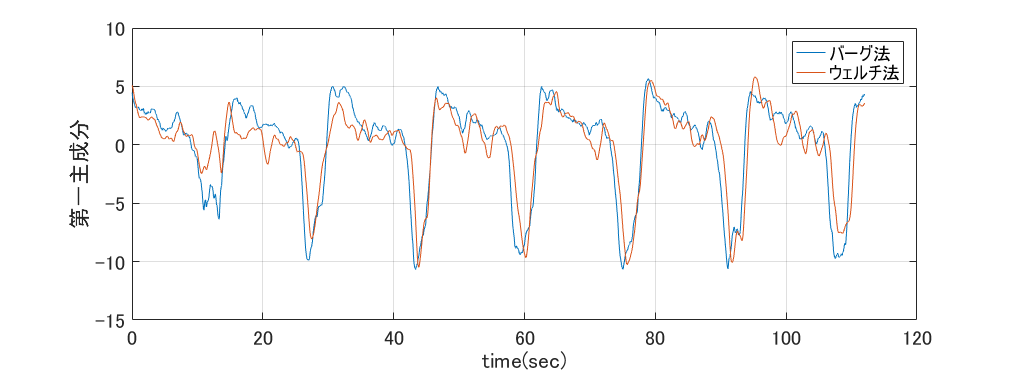
\includegraphics[width=13cm]{images/burgwelchPCA.png}
    \caption{第一主成分の比較}
    \label{fig:burgwelchPCA}
\end{figure}

また、分類としてもウェルチ法で得た特徴量が良い結果を出しており、
28の特徴量を用いた分類ではPCAを用いなくとも同等のAccuracyが得られている。
しかし、一方でLDAを用いてバーグ法の28の特徴量を入力として分類器の作成を行った場合、
テストデータに対して0.829、ウェルチ法を用いた場合には0.839の結果となり、
ウェルチ法を特徴量の方が僅かに良い結果だが、
特徴量と分類器の組み合わせに関して明確な指針が得られたとは言えない。

\subsection{畳込みニューラルネットワークを用いた分類}
次に畳込みニューラルネットワークを用いて次元削減と分類までを
一貫して行う手法を用いることとした。
スペクトル密度推定によって得た特徴量である\(x_i\)を28個並べた行列\(z_i=(x_i^T, x_{i+1}^T,\cdots, x_{i+27}^T)\ \in \mathbb R^{28\times 28}\)
を画像とみなし、畳込みニューラルネットワークの入力とする。

バーグ法によって抽出された28個の特徴量を用いた場合のテストAccuracyは0.871であり、
バーグ法による特徴を用いた場合で最高のAccuracyとなった(表\ref{table:accuracies}、ウェルチについては未実施)。

\begin{table}[t]
    \centering
    \caption{テストAccuracyの比較}
        \begin{tabular}{|c|c|c|} \hline
            分類手法\解析手法 & バーグ & ウェルチ \\ \hline
            LR &  0.729  & 0.849  \\ \hline
            PCA + LR & 0.842  & 0.843  \\  \hline
            LDA & 0.829  & 0.839  \\  \hline
            畳み込みNN & 0.871  &  \\ \hline
        \end{tabular}
    \label{table:accuracies}
\end{table}

\section{結論}
EEGからスペクトル解析によってERDを検出し、特徴量として用いることで
BCIの構築が可能である。また、パワースペクトル密度からERDを陽に検出できない場合でも
PCAによって潜在的に含まれていることを確認することができる。
また、スペクトル密度の時間変化を入力とした分類器を構築することで
足の動作を検知することが可能であると結論付けられ、
本実験では分類器として畳み込みニューラルネットワークが良い性能を出した。

しかし、特徴量や分類器の可能なすべての組み合わせから、
どのようなBCIの構成が最適であるかを知ることは困難である。
本実験のように各個人に対して
BCIを構築する場合はいくつかの組み合わせを検証することは可能であるが
商業利用が検討されているBCIが今後普及するためには、
EEGの解析と信号処理、機械学習の技術で個人事に逐一設計を行わなければならない方法では不十分である。

従ってEnd to End学習によるBCIの設計は重要な課題であると考えられる。
第\ref{chapter:myop}章以降、End to End学習に向けた研究について述べる。